% Options for packages loaded elsewhere
\PassOptionsToPackage{unicode}{hyperref}
\PassOptionsToPackage{hyphens}{url}
%
\documentclass[
]{book}
\usepackage{amsmath,amssymb}
\usepackage{iftex}
\ifPDFTeX
  \usepackage[T1]{fontenc}
  \usepackage[utf8]{inputenc}
  \usepackage{textcomp} % provide euro and other symbols
\else % if luatex or xetex
  \usepackage{unicode-math} % this also loads fontspec
  \defaultfontfeatures{Scale=MatchLowercase}
  \defaultfontfeatures[\rmfamily]{Ligatures=TeX,Scale=1}
\fi
\usepackage{lmodern}
\ifPDFTeX\else
  % xetex/luatex font selection
\fi
% Use upquote if available, for straight quotes in verbatim environments
\IfFileExists{upquote.sty}{\usepackage{upquote}}{}
\IfFileExists{microtype.sty}{% use microtype if available
  \usepackage[]{microtype}
  \UseMicrotypeSet[protrusion]{basicmath} % disable protrusion for tt fonts
}{}
\makeatletter
\@ifundefined{KOMAClassName}{% if non-KOMA class
  \IfFileExists{parskip.sty}{%
    \usepackage{parskip}
  }{% else
    \setlength{\parindent}{0pt}
    \setlength{\parskip}{6pt plus 2pt minus 1pt}}
}{% if KOMA class
  \KOMAoptions{parskip=half}}
\makeatother
\usepackage{xcolor}
\usepackage{color}
\usepackage{fancyvrb}
\newcommand{\VerbBar}{|}
\newcommand{\VERB}{\Verb[commandchars=\\\{\}]}
\DefineVerbatimEnvironment{Highlighting}{Verbatim}{commandchars=\\\{\}}
% Add ',fontsize=\small' for more characters per line
\usepackage{framed}
\definecolor{shadecolor}{RGB}{248,248,248}
\newenvironment{Shaded}{\begin{snugshade}}{\end{snugshade}}
\newcommand{\AlertTok}[1]{\textcolor[rgb]{0.94,0.16,0.16}{#1}}
\newcommand{\AnnotationTok}[1]{\textcolor[rgb]{0.56,0.35,0.01}{\textbf{\textit{#1}}}}
\newcommand{\AttributeTok}[1]{\textcolor[rgb]{0.13,0.29,0.53}{#1}}
\newcommand{\BaseNTok}[1]{\textcolor[rgb]{0.00,0.00,0.81}{#1}}
\newcommand{\BuiltInTok}[1]{#1}
\newcommand{\CharTok}[1]{\textcolor[rgb]{0.31,0.60,0.02}{#1}}
\newcommand{\CommentTok}[1]{\textcolor[rgb]{0.56,0.35,0.01}{\textit{#1}}}
\newcommand{\CommentVarTok}[1]{\textcolor[rgb]{0.56,0.35,0.01}{\textbf{\textit{#1}}}}
\newcommand{\ConstantTok}[1]{\textcolor[rgb]{0.56,0.35,0.01}{#1}}
\newcommand{\ControlFlowTok}[1]{\textcolor[rgb]{0.13,0.29,0.53}{\textbf{#1}}}
\newcommand{\DataTypeTok}[1]{\textcolor[rgb]{0.13,0.29,0.53}{#1}}
\newcommand{\DecValTok}[1]{\textcolor[rgb]{0.00,0.00,0.81}{#1}}
\newcommand{\DocumentationTok}[1]{\textcolor[rgb]{0.56,0.35,0.01}{\textbf{\textit{#1}}}}
\newcommand{\ErrorTok}[1]{\textcolor[rgb]{0.64,0.00,0.00}{\textbf{#1}}}
\newcommand{\ExtensionTok}[1]{#1}
\newcommand{\FloatTok}[1]{\textcolor[rgb]{0.00,0.00,0.81}{#1}}
\newcommand{\FunctionTok}[1]{\textcolor[rgb]{0.13,0.29,0.53}{\textbf{#1}}}
\newcommand{\ImportTok}[1]{#1}
\newcommand{\InformationTok}[1]{\textcolor[rgb]{0.56,0.35,0.01}{\textbf{\textit{#1}}}}
\newcommand{\KeywordTok}[1]{\textcolor[rgb]{0.13,0.29,0.53}{\textbf{#1}}}
\newcommand{\NormalTok}[1]{#1}
\newcommand{\OperatorTok}[1]{\textcolor[rgb]{0.81,0.36,0.00}{\textbf{#1}}}
\newcommand{\OtherTok}[1]{\textcolor[rgb]{0.56,0.35,0.01}{#1}}
\newcommand{\PreprocessorTok}[1]{\textcolor[rgb]{0.56,0.35,0.01}{\textit{#1}}}
\newcommand{\RegionMarkerTok}[1]{#1}
\newcommand{\SpecialCharTok}[1]{\textcolor[rgb]{0.81,0.36,0.00}{\textbf{#1}}}
\newcommand{\SpecialStringTok}[1]{\textcolor[rgb]{0.31,0.60,0.02}{#1}}
\newcommand{\StringTok}[1]{\textcolor[rgb]{0.31,0.60,0.02}{#1}}
\newcommand{\VariableTok}[1]{\textcolor[rgb]{0.00,0.00,0.00}{#1}}
\newcommand{\VerbatimStringTok}[1]{\textcolor[rgb]{0.31,0.60,0.02}{#1}}
\newcommand{\WarningTok}[1]{\textcolor[rgb]{0.56,0.35,0.01}{\textbf{\textit{#1}}}}
\usepackage{longtable,booktabs,array}
\usepackage{calc} % for calculating minipage widths
% Correct order of tables after \paragraph or \subparagraph
\usepackage{etoolbox}
\makeatletter
\patchcmd\longtable{\par}{\if@noskipsec\mbox{}\fi\par}{}{}
\makeatother
% Allow footnotes in longtable head/foot
\IfFileExists{footnotehyper.sty}{\usepackage{footnotehyper}}{\usepackage{footnote}}
\makesavenoteenv{longtable}
\usepackage{graphicx}
\makeatletter
\def\maxwidth{\ifdim\Gin@nat@width>\linewidth\linewidth\else\Gin@nat@width\fi}
\def\maxheight{\ifdim\Gin@nat@height>\textheight\textheight\else\Gin@nat@height\fi}
\makeatother
% Scale images if necessary, so that they will not overflow the page
% margins by default, and it is still possible to overwrite the defaults
% using explicit options in \includegraphics[width, height, ...]{}
\setkeys{Gin}{width=\maxwidth,height=\maxheight,keepaspectratio}
% Set default figure placement to htbp
\makeatletter
\def\fps@figure{htbp}
\makeatother
\setlength{\emergencystretch}{3em} % prevent overfull lines
\providecommand{\tightlist}{%
  \setlength{\itemsep}{0pt}\setlength{\parskip}{0pt}}
\setcounter{secnumdepth}{5}
\usepackage{booktabs}
\usepackage{amsthm}
\makeatletter
\def\thm@space@setup{%
  \thm@preskip=8pt plus 2pt minus 4pt
  \thm@postskip=\thm@preskip
}
\makeatother
\ifLuaTeX
  \usepackage{selnolig}  % disable illegal ligatures
\fi
\usepackage[]{natbib}
\bibliographystyle{apalike}
\usepackage{bookmark}
\IfFileExists{xurl.sty}{\usepackage{xurl}}{} % add URL line breaks if available
\urlstyle{same}
\hypersetup{
  pdftitle={Programming Logic for Non-Programmers},
  pdfauthor={Kat Koziar and Stephanie Labou},
  hidelinks,
  pdfcreator={LaTeX via pandoc}}

\title{Programming Logic for Non-Programmers}
\author{Kat Koziar and Stephanie Labou}
\date{2025-02-21}

\begin{document}
\maketitle

{
\setcounter{tocdepth}{1}
\tableofcontents
}
\chapter{About}\label{about}

\texttt{BEGIN\ pitch()}

Have you ever wondered how some of your colleagues can look at a computer programming script, with little prior knowledge of the language, and not only read it, but help fix the code? It's not because they know all programming languages, but because most programming languages use the same concepts and logic.

\texttt{STRUCTURE(workshop)}

In this interactive workshop, attendees will gain hands-on experience to understand and interpret programming logic. We will cover fundamental topics in programming including: conditional statements, loops, order of operations and logical flow, functions and arguments, and data types. Attendees will practice formulating programming arguments to accomplish common tasks, such as subsetting data based on a set of conditions.

\texttt{WHERE\ prior\_experience\ ==\ FALSE}

No coding experience required! Programming logic is transferable across specific languages, so learners will focus on concepts, rather than specific syntax from a specific language. Attendees will learn to interpret programming logic and build confidence to apply their understanding to various programming languages they may encounter.

\texttt{FOR\ (x\ in\ example1:example5)\ \{annotate(x)\}}

To provide real world examples of programming logic in practice, the workshop will integrate hands-on work time with examples of sample code written in R, Python, SQL, Stata, and other languages. Attendees will practice annotating code in human understandable language and discuss the process, and any pitfalls, with their peers and the instructors.

\texttt{IF\ attendee\_need\ ==\ “learn\_programming\_logic”:\ print(“register\ for\ this\ workshop!”)}

\chapter{Introduction}\label{intro}

This is a different type of programming workshop. One that doesn't require a computer, but instead intends to help you build mental models of how computer programming works. You will learn not only the logic behind programming, but also methods for identifying errors in algorithms and code that the computer doesn't see. The only technology required, besides the ability to view this lesson, is something to write with and a piece of paper.

\section{Building a Mental Model}\label{building-a-mental-model}

Our experience with computational consultations is often student researchers will take someone else's code and try to adapt it for their own research, but they use the code without knowing how it does what it does. This means they're unable to easily update the script, will create errors they don't know how to address, and even import errors already in the script. Sometimes they can't even adapt it to use the original data which is in a different location on their computer. They can't really read the code, but are reliant on the computer reading the code.

The purpose of this workshop isn't just to introduce you to programming logic, it's to provide a safe space to practice thinking through what the computer does by tracing algorithms and code snippets instead of having the computer just do it.

\section{A Note on Syntax}\label{a-note-on-syntax}

Syntax is the formal structural of a computer programming language. Assembly, C/C++, C\#, Python, and R all have formal language structures so the computer knows how to read the code. But, sometimes syntax gets in the way of learning concepts. Luckily, most programming concepts are the same across all languages.

The syntax we will use for most of the examples will be something called psuedocode. Pseudocode focuses on concepts and tasks, not syntax. You don't need to worry if there is a semicolon or parenthesis out of place when you write in psuedocode, you'll still know how to interpret what is written.

We will also introduce programming examples in different languages, so you can start to recognize the similarities and differences between the languages. You won't be an expert by end of this workshop, but we will help you build your skillset so hopefully you're more comfortable reading known (and unknown) computer languages.

\chapter{Algorithms}\label{algorithms}

Most people have heard the term algorithm, especially in relation to AI or social media feeds, but what is an algorithm? An algorithm is a set of instructions for how to do something. For AI, the term algorithm is often used as a term to represent the overall way that whatever AI that you're working with was trained to do what it does. For social media feeds, an algorithm will determine how to select which content is delivered to a user. Algorithms can be very simple or very complex.

A common analogy for an algorithm is a recipe. A recipe includes a set of ingredients, which are like the variables in your code, then lists instructions on what to do with the ingredients. But, a big difference between common recipes that you are used to seeing and an algorithm is you have to be very exact and specific when you tell a computer to do something. It isn't enough to tell a computer, ``get the data.'' You have to tell it where the data is located, what format it is in, how to read it, and what format you want the data in for use in your script. So let's do an example with a recipe on how to make cheesy mashed potatoes.

The steps are easy enough.
1. Take potatoes and boil them until they're done.
2. Drain.
3. Add butter, milk, salt/pepper to taste.
4. Mash.
5. Fold in cheese.
6. Eat.

Most of us would know how to do this because we infer the instructions that are missing. But, computers are stupid. They need to be explicitly told how to do something.

How many potatoes? What does \emph{boil} mean? What does \emph{done} mean? (which is also a question I asked my mom when reading my grandmother's recipes.)

Ingredients
3 pounds russet potatoes, peeled and cut into chunks
8 tablespoons (1 stick) butter
1/2 cup milk
Salt and freshly ground pepper
1 cup shredded cheddar

\emph{Algorithm for making Cheesy Mashed Potatoes}

\begin{enumerate}
\def\labelenumi{\arabic{enumi}.}
\tightlist
\item
  Place the potatoes in a large pot and cover with water by an inch. Bring to a boil over high heat, then reduce to simmer. Cook until the potatoes are fork tender, 25 to 30 minutes. Drain.
\item
  Return the potatoes to the pot and add the butter, milk and some salt and pepper. Mash the potatoes to the desired consistency. While still hot, fold the cheese into the mash and stir to melt.
\end{enumerate}

\section{Breakout Activity}\label{breakout-activity}

For this activity, you will write an algorithm to make popcorn.~

Sounds simple, right? ``Make popcorn'' is something most people have at least a general understanding of how to do. But in this scenario, you're providing step-by-step directions for a computer to understand how to make popcorn and a computer would need to be told \textbf{every action} to take, in order to successfully make popcorn.\\

Your task is to write out each step needed to make popcorn.

As you write out the steps with your group, consider:

\begin{itemize}
\tightlist
\item
  Are you opening a container at any point?
\item
  Are you making microwave popcorn, or using a stove?
\item
  How much time is needed to make popcorn?
\item
  What should the computer do if the popcorn starts burning?
\end{itemize}

\chapter{Data types}\label{data-types}

A word that people use a lot when referring to computer code is \emph{variables}, but what is a variable? A variable is a placeholder for some type of data that will be used in computer code.

\texttt{ingredients\ \textless{}-\ cheddar\ cheese,\ potatoes,\ milk,\ salt,\ butter}

We use variables to represent the data that are being used to because it's easy to change it,

\texttt{ingredients\ \textless{}-\ smoked\ gouda\ cheese,\ potatoes,\ milk,\ salt,\ butter}

and also easy to build a mental model of how the different variables interrelate.

A most simple example of this is to use variables to describe an equation. A common rule for naming variables is they should represent what the data are.

talk about data types and variables.

data types and data structures.

use food analogy

\section{Exercise - Who knows}\label{exercise---who-knows}

\chapter{Loops}\label{loops}

Drawing from Introduction to Programming Logic\citep{lynne_ohanlon_introduction_2000}
Start with \texttt{for} loop as first function term
``Populate an array from a for loop'' as an early example; pg 376 blank table with good early exercise.
Side note about infinite loop, importance of settling bounds
What happens if you don't tell loop to increase?
Examples of \texttt{for} loops in multiple languages (Python, C, R)?
To decide: all theory and then all practice, or theory/practice/theory/practice?
Also writing out result of each iteration otherwise you'll only get the last result (a common problem)

\section{Exercise - loop trace}\label{exercise---loop-trace}

Grab a pen and paper and write out the output of each iteration of the loop:

\begin{verbatim}
for x in 0 to 5 
  write x
  
\end{verbatim}

Loop output

0\\
1\\
2\\
3\\
4\\
5\\

\hfill\break

\section{Exercise - populate an array}\label{exercise---populate-an-array}

Let's use a \texttt{for} loop to populate an array.

We'll start with an empty array called \texttt{table} with 4 rows and columns named A, B, C, D, and E:

\begin{longtable}[]{@{}lllll@{}}
\toprule\noalign{}
A & B & C & D & E \\
\midrule\noalign{}
\endhead
\bottomrule\noalign{}
\endlastfoot
~ & ~ & ~ & ~ & ~ \\
~ & ~ & ~ & ~ & ~ \\
~ & ~ & ~ & ~ & ~ \\
~ & ~ & ~ & ~ & ~ \\
\end{longtable}

We want to populate this table with numbers, starting with 1 and increasing sequentially (1, 2, 3, 4, etc.). We want to fill each row completely before moving on to start filling the next row.

Our \texttt{for} loop:

\textbf{{[}{[}adapt programming logic book exercise for loop{]}{]}}

Grab and pen and paper (or a spreadsheet program like Google Sheets or Excel) and manually fill in the empty cells in the array.

\begin{itemize}
\tightlist
\item
  What is the number in cell A1?
\item
  What is the number in cell B2?
\item
  What is the number in cell D4?
\end{itemize}

Your filled array should look like this

\begin{longtable}[]{@{}lllll@{}}
\toprule\noalign{}
A & B & C & D & E \\
\midrule\noalign{}
\endhead
\bottomrule\noalign{}
\endlastfoot
1 & 2 & 3 & 4 & 5 \\
6 & 7 & 8 & 9 & 10 \\
11 & 12 & 13 & 14 & 15 \\
16 & 17 & 18 & 19 & 20 \\
\end{longtable}

\section{Other Types of Loops}\label{other-types-of-loops}

There are other types of loops in addition to the commonly used \texttt{for} loop.~

The \texttt{while} loop uses a condition at the start of the loop to determine, in advance, when the loop will stop. For example, recall the initial for loop:

\begin{verbatim}
for x in 0 to 5 
  write x
  
\end{verbatim}

An equivalent \texttt{while} loop would look like:

\begin{verbatim}

\end{verbatim}

Another type of loop is a \texttt{do\ while} loop (check at end) and an \texttt{until} loop (check at end).

\begin{verbatim}
\end{verbatim}

\begin{verbatim}
\end{verbatim}

\section{Caveats}\label{caveats}

Loops are a frequently encountered concept in programming and come with their own set of common issues.

\subsection{Infinite loops}\label{infinite-loops}

When condition is never false or otherwise has no break

\subsection{Overwriting outputs}\label{overwriting-outputs}

\begin{verbatim}
for x in 0 to 5 
  answer = x

write answer
  
\end{verbatim}

\chapter{Conditionals and Making Choices}\label{conditionals-and-making-choices}

Many times in programming, we want to take a certain action only if a certain condition is satisfied.\\

To do this, we can use conditional statements. The most commonly used format of a conditional statement in programming is an \texttt{if} statement, which is often combined with an \texttt{else} statement.\\

This structure tells the program to check a condition and the next step depends on whether the condition is true, or false. We can think of this as a narrative statement: ``If condition A is true, do action X. If condition A is not true, do action Y.''\\

In programming format, this narrative statement would look like:

\begin{verbatim}
IF conditionA == TRUE, do X
ELSE do Y
\end{verbatim}

Note that \texttt{else} here is used equivalent to ``if not true'', meaning \texttt{A\ ==\ FALSE}.\\

We are not limited to a single \texttt{TRUE}/\texttt{FALSE} check in an \texttt{if\ else} statement, where actions are limited to ``x if true, y in all other scenarios''.

The \texttt{else\ if} (written as \texttt{elif} in some programming languages) concept allows us to add another sequential check if the \texttt{if} statement is not true. Our updated narrative statement might be: ``If condition A is true, do action X. If condition B is true, do action Z. If neither condition A or condition B are true, do action Y.''\\

In programming format, this updated narrative statement would look like:

\begin{verbatim}
IF conditionA == TRUE, do X
ELSE IF conditionB == TRUE, do Z
ELSE do Y
\end{verbatim}

\section{Boolean Operators}\label{boolean-operators}

In programming, most things boil down to \texttt{true} or \texttt{false}. (Sometimes you may see true/false capitalized as \texttt{TRUE} and \texttt{FALSE}, but the concept is the same.)\\

Programming uses Boolean operators such as:\\

\begin{itemize}
\tightlist
\item
  \texttt{and} (may also see \texttt{\&} used)
\item
  \texttt{or} (may also see \texttt{\textbar{}} used)
\item
  \texttt{not} (may also see \texttt{!} to indicate negation, for instance \texttt{!=} for ``not equal'')
\item
  \texttt{equals} (also \texttt{==})

  \begin{itemize}
  \tightlist
  \item
    {[}SL note: most Boolean operator lists include AND, OR, NOT - should we include EQUALS here or keep as separate part of testing true/false?{]}
  \end{itemize}
\end{itemize}

\section{\texorpdfstring{Exercise - \texttt{ifelse} trace}{Exercise - ifelse trace}}\label{exercise---ifelse-trace}

Let's look at some examples of conditional statements in practice.

\begin{verbatim}
if x == y:
  print("values are equal")
else if x > y:
  print("x greater than y")
else:
  print("x must be less than y")
  
\end{verbatim}

For the first trace, we will set the values of \texttt{x} and \texttt{y} as:

\begin{verbatim}
x <- 37
y <- 42
\end{verbatim}

What will be the printed output from this \texttt{ifelse} section?\\

Answer

x must be less than y

\hfill\break

What if we reset \texttt{x} and \texttt{y} to:

\begin{verbatim}
x <- 75
y <- 9
\end{verbatim}

Answer

x greater than y

\hfill\break

\section{Caveats}\label{caveats-1}

\subsection{Order of operations}\label{order-of-operations}

Order of operations is critical for conditionals. The computer will go through each condition \textbf{in order}, so if an early condition is satisfied, the statement will conclude there and not check the other conditions.

\textbf{{[}{[}insert example here{]}{]}}

\subsection{Matching parentheses}\label{matching-parentheses}

For complex nested conditionals, be sure to use parentheses, and be sure parentheses are matched properly.

The code below, without a closing parentheses after ``equal'', will continue to expect input.

\begin{verbatim}
if (x == y) 
  print("values are equal"
  
\end{verbatim}

As far as the programming language is concerned, you haven't finished this \texttt{if} statement. So, it will wait to run until you have ``completed your thought'', so to speak, and provided the syntax (here, \texttt{)}) indicating that this statement is complete and the program is ready to run.

Alternately, if you have mismatched parentheses, the result may be an error.

\begin{verbatim}
if (x == y) 
  print("values are equal"))
  
\end{verbatim}

In this case, there is an extra closing parentheses \texttt{)} after \texttt{print("values\ are\ equal")} that doesn't have a matching \texttt{(} anywhere in the statement. The resulting error would look like:

\begin{verbatim}
Error: unexpected ')' in:
"if (x == y) {
    print("values are equal"))"
    
\end{verbatim}

\subsection{Formatting may vary}\label{formatting-may-vary}

Programming languages may have specific formatting for conditional statements. This may mean certain brackets must be used, new lines are required between sections, or tab indents are needed.

For example, Python expects \texttt{:} at the end of each section of an \texttt{ifelse} statement, uses \texttt{elif} for \texttt{else\ if}, and requires indentation to indicate action of each section:

\begin{verbatim}
if x == y:
  print("values are equal")
elif x > y:
  print("x greater than y")
else:
  print("x must be less than y")
\end{verbatim}

In contract, R makes use of curly brackets \texttt{\{\}} to indicate each section of an \texttt{ifelse} statement and while indentation is a convention for readability, it is not technically required for the code to run:

\begin{verbatim}
if (x == y) {
  print("values are equal")
} else if (x > y) {
  print("x greater than y")
} else {
  print("x must be less than y")
}
\end{verbatim}

\textbf{{[}{[}Note to self: add another 1 or 2 language examples here to show similarities and differences in formatting{]}{]}}

\chapter{Functions}\label{functions}

A ``function'' in programming is a piece of code that does a specific task.

Consider the example of calculating the mean of a set of values. On the one hand, you could write out code to manually add each value and divide by the number of values.\\

\begin{verbatim}
values = (2, 4, 7, 5, 9)

mean_value = (2 + 4 + 7 + 5 + 9) / 5
\end{verbatim}

\hfill\break
On the other hand, if you plan to take the mean of a set of values often, it would be easier to have a function that could do this task without you needing manually write it out every time.

\begin{verbatim}
[SL:insert pseucode to calculate mean without using sum() or len(), use a for loop maybe to call back? although I keep coming back to using len() at least...]
\end{verbatim}

\section{Arguments}\label{arguments}

In a function, ``arguments'' are the inputs that you can specify. So for a \texttt{mean()} function, the primary argument would be what kind of input to put in: \texttt{mean(x)} where \texttt{x} is a list or vector of values. Another argument might be an option for how to handle missing or \texttt{NA} values: \texttt{mean(x,\ na.rm\ =\ FALSE)} where the default value of \texttt{na.rm} is \texttt{FALSE}, indicating that \texttt{NA} values will \emph{not} be removed from the calculation. Optional arguments like this may come with a pre-supplied default, in this case that \texttt{na.rm\ =\ FALSE} and any \texttt{NA}values will be retained, unless this argument is manually changed to \texttt{TRUE}.\\

It is important to understand (a) what arguments are in a function and (b) what arguments are optional and what the defaults are. A function will run as long as the non-optional arguments are completed (that is, input is specified), but the resulting output may not match expectations unless you understand what other optional arguments were included, and what the default values were.\\

For example, let's return to the \texttt{mean()} function where our arguments are input (mandatory) and handling of \texttt{NA} values (optional).

If we only input the mandatory argument of specifying input:

\begin{verbatim}
values <- c(2, 4, 7, 5, 9, NA)
mean(values)
\end{verbatim}

The output of this function would be \texttt{NA}, because if we retain the \texttt{NA} values - which we do by default in the \texttt{mean()} function, then the mean will necessary be \texttt{NA}. For a computer, the sum of a set of values plus \texttt{NA} will always be \texttt{NA}, and taking the mean of \texttt{NA} will also return \texttt{NA}.

Conversely, if we specify that we want to remove \texttt{NA} values from our mean calculation:

\begin{verbatim}
values <- c(2, 4, 7, 5, 9, NA)
mean(values, na.rm = TRUE)
\end{verbatim}

Now our output is \texttt{5.4} which is the mean of \texttt{values} exlucding \texttt{NA}.

\section{Libraries}\label{libraries}

Programming languages will have a variety of functions for common tasks ready to use without any additional work. These are called ``built in'' functions and are available to use right away.\\

However, built in functions are often limited to basic tasks and do not include more complex or custom functions that you may with to use. Now, you can code more complex functions yourself, building off of the built in functions, but this would take a lot of time and require more in-depth programming knowledge.

The good news is that most programming languages will have optional ``libraries'' (or packages, or modules, depending on what term your programming language of choice uses) that include additional functions, beyond the built in function. So before creating a new function from scratch, it is worthwhile to check whether a library exists that includes a function that does what you want to do.\\

You can think of programming libraries as serving a role similar to actual libraries. For instance, you don't need to memorize every historical event, or write your favorite novel from scratch - you can check out a book from a library to read and learn more!\\

In the same way, your computer and your programming language of choice doesn't need to always have every single function on hand, which would take up a lot of space. Instead, it can ``check out'' (load) a ``book'' (collection of functions) created by another person. You can then use those additional functions the same way you would any function.\\

This set up saves computer disk space, ensures you don't have to recreate the wheel and make every function from scratch, and provides a level of standardization (e.g., everyone uses the same reference ``book'' so output should be the same for the same input, across users).\\

A good rule of thumb is if it \emph{seems} like the function you want is broadly useful, then someone has likely created a library containing it. This is also true for niche or domain-specific functions: if the task is one that comes up a lot in analysis, there is likely a library that has functions for those analysis tasks.\\

Finding the `right' library for the function you need can be overwhelming, but a good starting point is the official library collection for a programming language, such as \href{https://cran.r-project.org/web/views/}{CRAN for R} or \href{https://pypi.org/}{PyPI for Python}.

\section{Accessing functions in libraries}\label{accessing-functions-in-libraries}

The syntax for accessing functions in libraries varies by programming language but follows the general process of:

\begin{enumerate}
\def\labelenumi{\arabic{enumi}.}
\tightlist
\item
  Install the library from the source. You only need to do this once.
\item
  Load or import the library. You will need to do this every time you want to access a function in a library. By convention, libraries are loaded at the top of a script, so you, and other people, can see at a glance what libraries are needed to run the script.
\item
  Use the functions as normal.
\end{enumerate}

\subsection{Caveats}\label{caveats-2}

\subsection{Function names}\label{function-names}

There are only so many function names that make sense in the English language, so there may be functions from \emph{different libraries} that have the same name. How does the programming language know which function you are trying to access? By default, the language will use the function of the more recently loaded or imported package.

Let's say we have two \texttt{mean()} functions, one from library \texttt{A} and one from library \texttt{B}. They differ in their default settings:

\begin{itemize}
\tightlist
\item
  library \texttt{A} defauls to \texttt{na.rm\ =\ TRUE}
\item
  library \texttt{B} defaults to \texttt{na.rm\ =\ FALSE}
\end{itemize}

If we load libraries in order \texttt{A} then \texttt{B} and then use \texttt{mean()} as a function, we will be using the \texttt{mean()} function from library \texttt{B}.

\begin{verbatim}
load(A)
load(B)

values <- c(2, 4, 7, 5, 9, NA)
mean(values)
\end{verbatim}

Our result will be \texttt{NA}.

Conversely, if we load library \texttt{B} then library \texttt{A}, we will use the \texttt{mean()} function from library \texttt{A}.

\begin{verbatim}
load(B)
load(A)

values <- c(2, 4, 7, 5, 9, NA)
mean(values)
\end{verbatim}

Our value will be \texttt{5.4}.

The tricky part is that all this happens invisibly. There may or may not - depending on your programming language - be a warning that two libraries contain functions of the same name. So, keeping track of your order of loading is important. If you get any unexpected results, you can double check which library the function you are using is from.\\

An alternative method is to be explicit about which function you are calling. Most programming languages will allow a syntax along the lines of \texttt{library:function()} to specify use of a function from a stated library.\\

\begin{verbatim}
load(B)
load(A)

values <- c(2, 4, 7, 5, 9, NA)
B:mean(values)

#result will be `NA`
\end{verbatim}

\subsection{Aliases}\label{aliases}

You may encounter the concept of an ``alias'' for a library. This is common in Python, where users can set an alias for a library name, and use that going forward rather than writing out the full library name. This will mostly come up if you are looking for help online, or wondering why you are seeing abbreviations.

For example, Python uses the \texttt{import} term to load a library (or ``package'' as Python calls them) and allows setting an alias using \texttt{import\ package\ as\ alias} syntax. By convention, many Python users will use standard aliases for common packages, such as:

\begin{verbatim}
import pandas as pd
import numpy as np
\end{verbatim}

Functions can then be called using the explicit \texttt{package:function} syntax, such as \texttt{pd.DataFrame} to designate a \texttt{pandas} \texttt{DataFrame} object.

\section{Activity reprise for functions}\label{activity-reprise-for-functions}

Let's return to the Chapter 2 activity where you created an algorithm to make popcorn.

Call back to popcorn - if function is make\_popcorn - what is that for? What are your arguments - is it kernels or is it a bag, what time?
make\_popcorn(type = kernels, time = 15 minutes, butter = TRUE, salt = TRUE) vs make\_popcorn() with defaults
import cookbook; cookbook.make\_popcorn()
\#\#\# From stephanie import make\_popcorn()
\#\#\# From kat import make\_popcorn()

Libraries, packages, modules
Example: min (R), max (Python), mean (SQL), regression (R, Python, Stata)
Can look up documentation, most should specify arguments in each function and syntax, as well as defaults for arguments

\chapter{Comments and Names}\label{comments-and-names}

Concept of comments, naming of variables and variables
Briefly touch on common conventions (like \texttt{df} for dataframe); ask about disciplinary conventions for abbreviations or naming

{[}SL: kind of moved this into `caveats' of functions, flagged to discuss{]}

\chapter{Common Issues}\label{common-issues}

Some common issues

\section{\texorpdfstring{Difference between \texttt{=} and \texttt{==}}{Difference between = and ==}}\label{difference-between-and}

The former, \texttt{=} is used to set something as equal as in \texttt{x\ =\ 5} where
the variable \texttt{x} is equal to, or has a value of, \texttt{5}. Conversely, the
double equal \texttt{==} is used to test for equality. For instance, if we set
a variable x to equal the value 5, the code \texttt{x\ ==\ 5} would return \texttt{True}
and the code \texttt{x\ ==\ 6} would return \texttt{False}.\\

\section{Spelling and capitalization matter}\label{spelling-and-capitalization-matter}

The variable \texttt{x} is different from the variable \texttt{X}. Likewise, a
function \texttt{mean()} and a function \texttt{Mean()} would be separate functions.

\section{Special characters and words}\label{special-characters-and-words}

Many programming languages reserve specific words for specific tasks.
For example, a function called \texttt{sum()} is fairly common across
languages. While you \emph{could} make your own alternate function called
\texttt{sum()}, this may lead to unexpected results when using the \texttt{sum()}
function\\

Similarly, it is best practice to avoid naming variables or objects the
same as common function names. Again, while you \emph{could} write code like
\texttt{sum\ =\ sum()}, this will get confusing for you, and may lead to
unexpected results and code behavior downstream.

The same is true for certain characters. Many programming languages
treat \texttt{NA} as a special class of missing value. This is \emph{not} the same
as \texttt{"NA"}, which would instead be a character string containing the
letters NA.

\section{Ending a code chunk}\label{ending-a-code-chunk}

Ending a statement (needing ; or other conclusion)

\section{Order of operations}\label{order-of-operations-1}

overwriting/ variable will be whatever most recently set as

\section{Others {[}work in progress{]}}\label{others-work-in-progress}

Closing quotes and parenthese\\
Direct comparison of multiple syntax, so like the same task in R,
Python, C, SQL, Stata, Java~ You don't need to memorize specifics!
Reading and writing data / files\\
Syntax is going to be specific to a language, or package within a
language\\
Show some examples of reading/writing data in R, Python, Stata, SQL

\chapter{Practice annotating and understanding unfamiliar code}\label{practice-annotating-and-understanding-unfamiliar-code}

\section{\texorpdfstring{Nested \texttt{for} loops and \texttt{if\ else} statements (in Python)}{Nested for loops and if else statements (in Python)}}\label{nested-for-loops-and-if-else-statements-in-python}

Here is an example of code that is scraping content from a set of website pages and saving that content locally. It uses `nested' \texttt{for} loops, meaning a second loop occurs within the first loops. It also uses nested \texttt{if\ else} statements.

\textbf{SL: we can simplify this example, maybe remove session\_id and save\_loc}

For this code, can you identify where each \texttt{for} loop and each \texttt{if\ else} statement ends? Or put another way, can you figure out on which lines (numbered in code chunk below) each statement starts and stops?

\begin{verbatim}
1.  base_url = "https://nces.ed.gov/ipeds/datacenter/"
2.  data_url = "DataFiles.aspx?"
3.  year_base = "year="
4.  years = ["1995", "1996", "1997", "1998"]
5.  session_id = "&sid=4f8f293f-df75-42cd-9cc0-ed184270cf17&rtid=7"  #you might need to change this
6. 
7.  # what type of files do you want to save?
8.  file_type = ["zip","csv"]
9. 
10. # where do you want to save locally?
11. 
12. # save_loc is redundant, but a reminder that you should have locally folders that reflect the years, 13. because that's where below is saving to
14. save_loc = years 
15. 
16. # what kind of prefix do you want on your files
17. save_prefix = "ipeds_" 
18. 
19. # scrape
20. for year in years:
21.     url = base_url+data_url+year_base+year+session_id 
22.     webpage = requests.get(url)
23.     soup = BeautifulSoup(webpage.content, 'html.parser')
24. 
25. 
26.     if os.path.isdir("./"+year):
27.         # notice output path has "year" as a variable indicating folders
28.         output_path = "./"+year+"/"+save_prefix+year+"_"+".html"
29.     
30.         if os.path.exists(output_path):
31.             print(output_path+" already exists. Did NOT save.")
32.         else:
33.             # saving the html file
34.             print("saving "+output_path)
35.     
36.             with open(output_path, 'wb') as file:
37.                 file.write(webpage.content) 
38.             
39.         # saving files linked on original html page which meet file type requirement
40.         for link in soup.find_all('a')[0:16]:  
41.             data_target = link.get('href')
42.             # data_target[-3:]
43.             if any(extension == data_target[-3:] for extension in file_type):
44.                 wget_url = base_url+data_target
45.                 wget_save = "./"+year+"/"+save_prefix+data_target.replace("/","-")
46.     
47.                 if os.path.exists(wget_save):
48.                     print(wget_save+" already exists. Did NOT save.")
49.                 else:
50.                     print("SAVING "+ wget_url+ " at local location: "+wget_save)
51.                     wget.download(wget_url,wget_save)
52.                     time.sleep(.25) # be kind, don't look like a DDOS attack
53.     else:
54.         print("\n!!! save directory "+year+" does NOT exist. please create\n")
55.     
56.     
57. print("fin.")
\end{verbatim}

\section{New types of conditions (in SQL)}\label{new-types-of-conditions-in-sql}

Consider the following SQL command:

\begin{verbatim}
SELECT * FROM OceanBuoys
WHERE Ocean = 'Atlantic' AND (BuoyName LIKE 'S%' OR BuoyName LIKE 'K%');
\end{verbatim}

Your preferred approach for navigating and understanding unfamiliar code may vary.\\

One option is to break down code into its component parts. Here you can separate out functions (common tasks across programming languages) from data-specific variables and names. Can you identify:

\begin{itemize}
\tightlist
\item
  What does the \texttt{OceanBuoys} term most likely refer to?
\item
  What do you think the \texttt{SELECT} function does?
\item
  What does \texttt{*} indicate, in combination with \texttt{SELECT}?
\item
  Parsing the second line that starts with \texttt{WHERE}, can you make an educated guess about what \texttt{Country} and \texttt{BuoyName} refer to?
\item
  Can you guess (or feel free to use Google) what \texttt{LIKE\ \textquotesingle{}S\%\textquotesingle{}} and \texttt{LIKE\ \textquotesingle{}K\%\textquotesingle{}} would indicate?
\end{itemize}

Do your answers match these?

\begin{itemize}
\tightlist
\item
  The \texttt{OceanBuoys} term here refers to a table or dataframe.
\item
  The \texttt{SELECT} function selects columns from a table.
\item
  The \texttt{*} here indicates that we want to return all columns from the table.
\item
  The \texttt{OceanBuoys} table must have columns named \texttt{Country} and \texttt{BuoyName}.
\item
  \texttt{LIKE} is used for pattern matching. This code is matching values that start with ``S'' or with ``K''.
\end{itemize}

\hfill\break

Now, can you write out a narrative of what you see the code is trying to do?\\

Example written narrative

Starting from the \texttt{OceanBuoys} table, return all columns but only rows where \texttt{Country} is equal to ``Spain'' \textbf{and} where the \texttt{BuoyName} value starts with ``S'' or ``K''.

\hfill\break

\section{add example for C/C++}\label{add-example-for-cc}

\section{Challenge practice: new syntax and terms (in R)}\label{challenge-practice-new-syntax-and-terms-in-r}

While the logic underlying programming languages stays consistent, a central challenge is that different languages often have their own special syntax, which can take a while to get used to. But don't panic! Familiarity comes with experience and in the meantime, Google is your friend.\\

In the code example below, note the new symbol \texttt{\%\textgreater{}\%} and \texttt{\%in\%} and the new functions \texttt{mutate()} and \texttt{paste()}. The \texttt{select()} function at least is more familiar from the example above, and \texttt{ifelse} is an \texttt{if\ else} statement.

\begin{verbatim}
1.  df_new <- df %>% 
2.    select(-respondent_name) %>% 
3.    mutate(identifier = paste(respondent_id, survey_wave, sep = "_")) %>% 
4.    mutate(survey_type = ifelse(survey_wave %in% c("first", "second"), "phone", "in person"))
  
\end{verbatim}

Task: go line by line and annotate, in your own words, what that line of code is doing.\\

Each line has a new take on the same logic we've covered in prior sections; a breakdown of new terms is below, to guide your annotation.

\begin{itemize}
\tightlist
\item
  Line 1

  \begin{itemize}
  \tightlist
  \item
    What is \texttt{df\_new\ \textless{}-\ df} doing here?
  \item
    What does the \texttt{\%\textgreater{}\%} symbol indicate?
  \end{itemize}
\item
  Line 2

  \begin{itemize}
  \tightlist
  \item
    What is the \texttt{select()} function likely doing?
  \item
    What might it mean that the argument in this function is preceded by \texttt{-}?
  \end{itemize}
\item
  Line 3

  \begin{itemize}
  \tightlist
  \item
    Using context clues (and Google) what do you think the \texttt{mutate()} function does?
  \item
    The new \texttt{paste()} function has three arguments (\texttt{paste(arg1,\ arg2,\ arg3)}). What do you think the arguments are for?
  \end{itemize}
\item
  Line 4

  \begin{itemize}
  \tightlist
  \item
    This \texttt{ifelse()} statement has a different format than we've covered so far, but the concept is the same. Assuming this \texttt{ifelse()} statement has three arguments (\texttt{ifelse(condition,\ mystery1,\ mystery2)}) what might the two mystery arguments be specifying?
  \item
    Looking at the section \texttt{survey\_wave\ \%in\%\ c("first",\ "second")}, what do you think this would translate to, as a written explanation of the task here?
  \end{itemize}
\end{itemize}

Finally, it is always important to understand the data type and structure of the data being acted upon. Keep in mind, based on the questions above, what is the structure of the data being used here?

Example narrative

Starting from the table/dataframe called ``df'', we want to keep (select) all columns \emph{except} the column named ``respondent\_name''.\\

Then, make a new column called ``identifier''. This new column is created by pasting together the value in the ``respondent\_id'' column and the ``survey\_wave'' column, separated by an underscore.\\

Then, make another new column called ``survey\_type''. The values in this column are determined by an \texttt{ifelse} statement: if the value in the ``survey\_wave'' column is any of the values specified in the list \texttt{("first",\ "second")} (so if the value is ``first'' or ``second''), then the value in the ``survey\_type'' column will be ``phone''. Otherwise, the value will be ``in person''.\\

\hfill\break

\chapter{Recap and Consultation Tips}\label{recap-and-consultation-tips}

Recap - you won't be an expert, the idea is to build up your skillset

\section{Approaching Consultations}\label{approaching-consultations}

How you may approach consultations - prepare in advance knowing specific question, evening seeing code in advance; have student talk through their code
Be clear with what you can and cannot do.
Helping with programming vs statistics (for when they ask for help with interpreting something Full disclosure, I am not a statistician)
Troubleshooting vs consult
Ok to say you don't know! Point to documentation and learning resources

\section{Three Areas For Errors}\label{three-areas-for-errors}

Code not running at all → often a syntax error

Running unexpectedly / unexpected output

input

logic

output

\chapter{BD Demo Introduction}\label{bd-demo-intro}

\begin{quote}
Bookdown reference: \url{https://bookdown.org/yihui/bookdown/usage.html}
\end{quote}

You can label chapter and section titles using \texttt{\{\#label\}} after them, e.g., we can reference Chapter \ref{intro}. If you do not manually label them, there will be automatic labels anyway, e.g., Chapter \ref{bd-demo-methods}.

Figures and tables with captions will be placed in \texttt{figure} and \texttt{table} environments, respectively.

\begin{Shaded}
\begin{Highlighting}[]
\FunctionTok{par}\NormalTok{(}\AttributeTok{mar =} \FunctionTok{c}\NormalTok{(}\DecValTok{4}\NormalTok{, }\DecValTok{4}\NormalTok{, .}\DecValTok{1}\NormalTok{, .}\DecValTok{1}\NormalTok{))}
\FunctionTok{plot}\NormalTok{(pressure, }\AttributeTok{type =} \StringTok{\textquotesingle{}b\textquotesingle{}}\NormalTok{, }\AttributeTok{pch =} \DecValTok{19}\NormalTok{)}
\end{Highlighting}
\end{Shaded}

\begin{figure}

{\centering 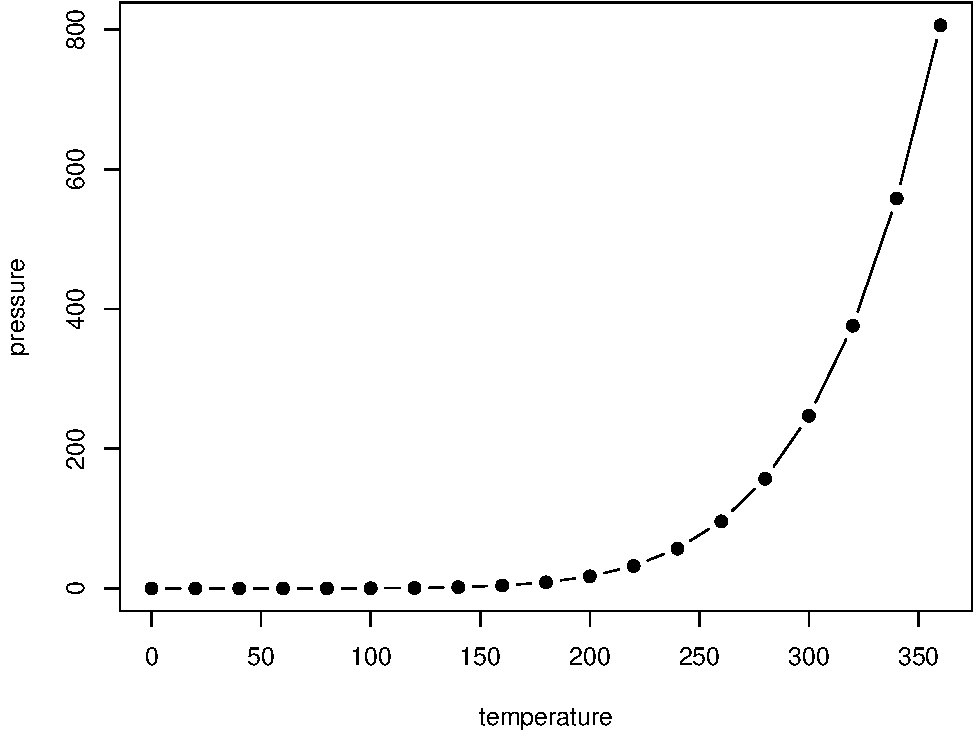
\includegraphics[width=0.8\linewidth]{programming-logic_files/figure-latex/nice-fig-1} 

}

\caption{Here is a nice figure!}\label{fig:nice-fig}
\end{figure}

Reference a figure by its code chunk label with the \texttt{fig:} prefix, e.g., see Figure \ref{fig:nice-fig}. Similarly, you can reference tables generated from \texttt{knitr::kable()}, e.g., see Table \ref{tab:nice-tab}.

\begin{Shaded}
\begin{Highlighting}[]
\NormalTok{knitr}\SpecialCharTok{::}\FunctionTok{kable}\NormalTok{(}
  \FunctionTok{head}\NormalTok{(iris, }\DecValTok{20}\NormalTok{), }\AttributeTok{caption =} \StringTok{\textquotesingle{}Here is a nice table!\textquotesingle{}}\NormalTok{,}
  \AttributeTok{booktabs =} \ConstantTok{TRUE}
\NormalTok{)}
\end{Highlighting}
\end{Shaded}

\begin{table}

\caption{\label{tab:nice-tab}Here is a nice table!}
\centering
\begin{tabular}[t]{rrrrl}
\toprule
Sepal.Length & Sepal.Width & Petal.Length & Petal.Width & Species\\
\midrule
5.1 & 3.5 & 1.4 & 0.2 & setosa\\
4.9 & 3.0 & 1.4 & 0.2 & setosa\\
4.7 & 3.2 & 1.3 & 0.2 & setosa\\
4.6 & 3.1 & 1.5 & 0.2 & setosa\\
5.0 & 3.6 & 1.4 & 0.2 & setosa\\
\addlinespace
5.4 & 3.9 & 1.7 & 0.4 & setosa\\
4.6 & 3.4 & 1.4 & 0.3 & setosa\\
5.0 & 3.4 & 1.5 & 0.2 & setosa\\
4.4 & 2.9 & 1.4 & 0.2 & setosa\\
4.9 & 3.1 & 1.5 & 0.1 & setosa\\
\addlinespace
5.4 & 3.7 & 1.5 & 0.2 & setosa\\
4.8 & 3.4 & 1.6 & 0.2 & setosa\\
4.8 & 3.0 & 1.4 & 0.1 & setosa\\
4.3 & 3.0 & 1.1 & 0.1 & setosa\\
5.8 & 4.0 & 1.2 & 0.2 & setosa\\
\addlinespace
5.7 & 4.4 & 1.5 & 0.4 & setosa\\
5.4 & 3.9 & 1.3 & 0.4 & setosa\\
5.1 & 3.5 & 1.4 & 0.3 & setosa\\
5.7 & 3.8 & 1.7 & 0.3 & setosa\\
5.1 & 3.8 & 1.5 & 0.3 & setosa\\
\bottomrule
\end{tabular}
\end{table}

You can write citations, too. For example, we are using the \textbf{bookdown} package \citep{R-bookdown} in this sample book, which was built on top of R Markdown and \textbf{knitr} \citep{xie2015}.

\section{Keeping this below for easy reference while we get used to the bookdown format}\label{keeping-this-below-for-easy-reference-while-we-get-used-to-the-bookdown-format}

\emph{Prerequisites}

This is a \emph{sample} book written in \textbf{Markdown}. You can use anything that Pandoc's Markdown supports, e.g., a math equation \(a^2 + b^2 = c^2\).

The \textbf{bookdown} package can be installed from CRAN or Github:

\begin{Shaded}
\begin{Highlighting}[]
\FunctionTok{install.packages}\NormalTok{(}\StringTok{"bookdown"}\NormalTok{)}
\CommentTok{\# or the development version}
\CommentTok{\# devtools::install\_github("rstudio/bookdown")}
\end{Highlighting}
\end{Shaded}

Remember each Rmd file contains one and only one chapter, and a chapter is defined by the first-level heading \texttt{\#}.

To compile this example to PDF, you need XeLaTeX. You are recommended to install TinyTeX (which includes XeLaTeX): \url{https://yihui.org/tinytex/}.

\chapter{BD Demo Methods}\label{bd-demo-methods}

We describe our methods in this chapter.

Math can be added in body using usual syntax like this

\section{math example}\label{math-example}

\(p\) is unknown but expected to be around 1/3. Standard error will be approximated

\[
SE = \sqrt{\frac{p(1-p)}{n}} \approx \sqrt{\frac{1/3 (1 - 1/3)} {300}} = 0.027
\]

You can also use math in footnotes like this\footnote{where we mention \(p = \frac{a}{b}\)}.

We will approximate standard error to 0.027\footnote{\(p\) is unknown but expected to be around 1/3. Standard error will be approximated

  \[
  SE = \sqrt{\frac{p(1-p)}{n}} \approx \sqrt{\frac{1/3 (1 - 1/3)} {300}} = 0.027
  \]}

  \bibliography{book.bib,packages.bib}

\end{document}
